% Chapter 60: Why Symmetry Breaks
\chapter{Why Symmetry Breaks}

\step{A Counterintuitive Opening}

\begin{mainline}
Carefully stand a pencil point-down on a smooth table. Before releasing it, answer one question: which way will it fall?

The table is level and gravity points straight down. East, south, west, and north have no special status. Newtonian mechanics and gravity, the pencil's governing laws, treat all horizontal directions equally. Yet falling inevitably selects one direction. Who chooses for it?

Now consider a refrigerator magnet. Iron atoms' tiny internal magnetic needles resemble countless miniature compasses; electromagnetism likewise favors no spatial direction. Yet this magnet firmly distinguishes north and south and holds your note. Directionless laws produce a directed magnet.

Chapter~57 defined symmetry as unchanged laws after a change; Chapter~58 showed how Noether's theorem produces conservation laws from symmetry. If symmetry is so powerful, why is the world not completely uniform, structureless porridge? Galaxies have spiral arms, snowflakes six branches, magnets poles, and pencils falling directions. Where do these preferences originate?

We ask why symmetric laws generate an asymmetric world. The answer unfolds in three steps: identify symmetry's level, see why a symmetric state becomes untenable, and discover how temperature, pressure, and load switch breaking on and off. Pencils, magnets, snowflakes, liquid-crystal screens, and even elementary-particle masses will tell the same story.
\end{mainline}

\step{Make a Guess First}

\begin{mainline}
Write three predictions as specifically as possible. Only explicitly stated intuition can be contradicted by experiment; a vague ``probably'' can never lose and therefore never learn.

First, if you balance the same pencil a hundred times, will falling directions spread uniformly or favor one side?

Second, imagine a perfectly ideal pencil: a mathematical point tip, an absolutely level table, motionless air, and no vibration. Will it stand forever?

Third, heat a magnet until red-hot and let it cool. How does its magnetism change? Will its poles still point the original way afterward?

% BEGIN TRANSLATOR SAFETY NOTE
\textbf{Translator safety note:} Do not heat magnets, refrigerator magnets, or unknown magnetic materials in a flame. Heat can damage coatings and materials, and neodymium magnets can ignite under unsuitable heating. Use a recorded Curie-temperature demonstration; see \href{https://www.kjmagnetics.com/faq.asp}{K\&J Magnetics' manufacturer guidance on heating magnets}.
% END TRANSLATOR SAFETY NOTE

Most intuitions say roughly uniform, forever upright, and magnetism disappearing then returning in an arbitrary direction. One is basically right; one is barely right classically but wrong in reality; and one hides a temperature watershed. Return afterward to grade your intuition.
\end{mainline}

\step{Hands-on Experiment}

\begin{experiment}[Balance a Pencil a Hundred Times (Twenty Will Do)]
\textbf{Materials:} a pencil or chopstick, white paper, and a pen.

\textbf{Procedure:}
\begin{enumerate}[leftmargin=2em]
  \item Draw a small circle in the paper's center and eight compass-direction marks around it.
  \item Stand the pencil centrally, as vertically as possible, release it, and record its falling direction.
  \item Repeat at least twenty times, using the same setup each time without deliberately favoring a direction.
  \item Mark each fall on the compass and count marks in each direction.
\end{enumerate}

\textbf{What you will see:} no single direction is predictable, but the points spread roughly uniformly with no clear favorite. Occasionally the pencil remains upright, usually because a blunt tip or tiny tabletop dent traps it in a shallow hollow.

\textbf{First extension:} sandwich the pencil between two books so it can fall only within a vertical slit. Adjust the confinement and feel how nearer-perfect centering extends its stay, while once falling starts it accelerates. Remember this feeling: it is the chapter's mathematical picture.

\textbf{Second extension:} stand a plastic ruler with one end against the table and press vertically downward on the other with your finger. Slowly increase force and notice two things: it resists for quite a while before bending, then suddenly springs to one side above a certain load, with the side hard to predict. Repeat to feel how rules choose no side but results must choose one.

% BEGIN TRANSLATOR SAFETY NOTE
\textbf{Translator safety note:} Do not force a plastic ruler to buckle or snap: it can spring outward or produce fragments. Use a video or instructor-designed restrained demonstration instead. Keep faces away from any loaded apparatus; see \href{https://www.osha.gov/eye-face-protection}{OSHA guidance on mechanical eye and face hazards}.
% END TRANSLATOR SAFETY NOTE
\end{experiment}

\begin{mainline}
Record three observations: individual outcomes are unpredictable; many outcomes have a symmetric statistical distribution; and the central position exists but cannot be maintained. The third unlocks the chapter.
\end{mainline}

\step{The Old Model Runs into Trouble}

\begin{mainline}
Several seemingly reasonable old ideas cause trouble when placed together.

First: symmetric causes yield symmetric results. If laws treat directions equally, results should have no preference. The pencil refutes this: symmetric cause, asymmetric outcome.

Second: asymmetric results require prior external asymmetry---wind, an uneven table, or a shaking hand. This seems airtight, but however small the disturbance becomes, with evacuated air, laser leveling, or robotic release, the pencil still falls with randomly uniform direction. Disturbances choose which fall goes which way, not why falling is unavoidable.

Third: Chapter~58 links rotational symmetry to angular momentum conservation. The falling pencil clearly rotates in one direction; has angular momentum appeared from nowhere? Account carefully: it acquires a small angular momentum related to falling direction, originating in amplified initial random displacement. Pencil plus Earth still conserves total angular momentum, and uniformly distributed repeated falls average to zero. Conservation survives; the stronger assumption that each individual result must share the laws' symmetry does not.

A subtler fourth idea says sufficiently precise initial conditions determine everything, so unpredictability only reflects measurement limits. This is true within classical mechanics but hides quantitative hopelessness. We will estimate that falling time grows only logarithmically with initial precision: shrinking initial displacement ten thousandfold buys less than one extra second. A hundred-millionfold improvement buys little predictability. Unstable systems amplify initial conditions without limit rather than merely being fussy about them, making exact specification practically empty words.

The real problem is conflating \textbf{symmetry of laws} with \textbf{symmetry of states}. Rotationally invariant equations need not have individually invariant solutions. Resolving a contradiction often begins with inventing a distinction between levels.
\end{mainline}

\step{Inventing New Concepts}

\begin{mainline}
Let us build the concepts one by one as physicists do.

\textbf{First distinction: symmetric laws permit asymmetric states.} Governing equations possess rotational symmetry but allow many solutions, each potentially asymmetric. The upright pencil is a symmetric but unstable solution; the eastward-fallen pencil is asymmetric but comfortably stable. The world lives in solutions, not equations.

\textbf{Second concept: unstable equilibrium.} A ball can rest atop a hill with balanced forces, yet a hair's-width displacement grows ever larger. A symmetric hilltop exists mathematically but effectively not physically. The upright pencil and a magnet's magnetization direction above its Curie temperature are such symmetric states: present but untenable.

\textbf{Third concept: degeneracy.} A pencil fallen east, south, west, or north has the same low energy. There is a whole family of equivalent lowest-energy states, not one: degeneracy. The system must settle into one with no reason to prefer any; all are equivalent.

\textbf{Central definition: spontaneous symmetry breaking.} When the actual state, usually the lowest-energy state, lacks some symmetry of the governing laws, symmetry is \textbf{spontaneously broken}. Spontaneous is crucial: no external force makes the decision; asymmetry grows from instability itself.

\textbf{Control case: explicit breaking.} Push the pencil over or magnetize iron with an external field, and the environment first breaks the rules while the system obeys. This ordinary explicit breaking is not our focus; we care about cases without a pusher.

\textbf{A measure: order parameter.} We need a quantity recording what was chosen and how firmly. For magnets it is magnetization, the alignment of tiny needles per unit volume. Zero in the symmetric phase and nonzero in the broken phase, it has meaningful direction and magnitude. Such quantities are order parameters.

\textbf{An arbiter: temperature and phase transition.} Magnetization is temperature's verdict, not destiny. Heat iron above about \(1043\ \mathrm{K}\), or \(770\ ^{\circ}\mathrm{C}\), its Curie temperature, and thermal agitation overwhelms mutual alignment, erasing magnetism and restoring symmetry. Cool through it and the symmetric state becomes unstable again; magnetism appears spontaneously. A definite temperature boundary separates symmetry and breaking: a phase transition.

\textbf{Final distinction: discrete versus continuous breaking.} An upright released coin ends heads or tails up: a discrete choice between two forks. A pencil can fall anywhere around a full circle: continuous choice. This is more than a numerical difference. Continuous breaking brings something discrete breaking lacks: a slow fluctuation costing almost no energy. Spin waves in magnets and sound in solids embody it; the coin has no corresponding soft mode.

Two more examples broaden the concepts. Break a round soda cracker and it splits along one crack. Approximately isotropic material and loading produce a particular fracture direction, though manufactured weak points make the choice less free. In Gulliver's Travels, Lilliput wars over breaking eggs at the big or little end. Both choices are equivalent under the rules, yet a society's chosen end hardens into tradition: a social version of broken states with symmetric laws.

A final everyday analogy: at a round-table banquet, each guest has a glass on either side and may take only their own, though the rule cannot distinguish left from right. Once the first guest takes the left glass, everyone follows and the direction is fixed. \textbf{What it resembles:} symmetric rules, broken outcomes, and a tiny first action setting the global direction. \textbf{What it does not:} the first guest has real preferences and arms, a genuine external cause. Physical spontaneous breaking needs no biased pusher: the symmetric state is itself unstable. Stop the analogy here; a banquet is not the mechanism.
\end{mainline}

\step{A One-Sentence Model}

\begin{oneline}
Laws are impartial, but the world lives in solutions: symmetric equations permit a whole family of equivalent asymmetric solutions, and an actual state must inhabit one. Symmetry does not disappear; it retreats from each state into the collection of all possible states.
\end{oneline}

\begin{mainline}
Split this into three parts. Symmetric equations: rotate the table and pencil equations stay unchanged. Symmetric solution set: the circle of all possible falling directions is rotationally invariant. Asymmetric individual solution: each fall points somewhere definite. Spontaneous breaking means symmetry changes its address, not that it vanishes.

In Chapter~57's language, physics asks not whether something looks uniform but whether transformations change its laws. After breaking, rotation maps one solution to another while the whole set and governing laws remain untouched. Symmetry's probe targets the larger object, laws plus every possible state, never a lone state. Our puzzle then dissolves: asymmetric states and symmetric laws occupied different levels from the beginning and cannot overthrow one another.
\end{mainline}

\step{The Mathematical Translator}

\begin{mainline}
Draw our hilltops and valleys. A variable \(x\) represents state: pencil displacement or magnetization as order parameter. A curve \(V(x)\) gives potential energy at \(x\). Like a ball rolling on the curve, the system always heads downward.

The symmetric phase is a bowl with a unique central minimum, \(x=0\), where the symmetric state rests stably. The broken phase raises a central bump and splits the bottom into two symmetric valleys. The center stays put but turns from valley into hilltop. One simple expression produces both:
\[
V(x)=a\,x^{2}+b\,x^{4}\qquad (b>0).
\]
The left gives energy at \(x\). On the right, the first term raises or lowers the center; the second makes distant sides rise steeply so the system cannot run to infinity.

Check special cases immediately. For \(a>0\), the \(x^{2}\) term dominates and \(x=0\) is the sole valley: symmetric phase. For \(a<0\), the center becomes a hill with valleys at \(x=\pm\sqrt{-a/(2b)}\), two equivalent broken states. At \(a=0\), valleys return to center and flatten, the transition's critical point. If \(b\) also becomes zero or negative, \(V(x)\) falls without limit as \(|x|\) grows, losing stable minima; the failed model needs higher-order terms. As \(a\) changes continuously from positive to negative, valley position \(\sqrt{-a/(2b)}\) grows continuously from zero. Breaking is continuous, matching magnetization's continuous rise near the Curie temperature.

This energy landscape is more general than it looks. Two examples reveal the same parameter-sign-change and central-instability framework.

\textbf{Engineering breaking: column buckling.} Stand a plastic ruler against a table and press down. Under small load it remains straight, a symmetric solution; beyond a critical load it suddenly bends sideways. Left and right have equal energy, equations favor neither, and minute initial curvature determines the result. Structural engineers call this buckling. Scaffold uprights, bridge struts, and thin rocket-tank shells all have a critical load destabilizing the straight solution, requiring ample design margins. Load controls \(a\): increasing it turns \(a\) from positive to negative and straightness from valley to hilltop.

% BEGIN TRANSLATOR SAFETY NOTE
\textbf{Translator safety note:} Treat this ruler example as a description, not a repeat instruction. Use a video or purpose-designed restrained apparatus; a loaded ruler can spring outward or break. See \href{https://www.osha.gov/eye-face-protection}{OSHA guidance on mechanical eye and face hazards}.
% END TRANSLATOR SAFETY NOTE

\textbf{Screen breaking: liquid-crystal displays.} Liquid-crystal molecules resemble tiny molecular pencils. At high temperature they point randomly, treating directions equally. Below a transition they spontaneously share an approximate orientation, breaking rotation symmetry; molecular orientation is the order parameter. Engineers exploit electrical control of this orientation. Each phone pixel is an artificially controlled broken phase: fields collectively turn molecules, altering transmitted polarized light and therefore brightness. Every lit screen repeatedly manipulates spontaneous breaking across hundreds of thousands of pixels.
\end{mainline}

\begin{center}
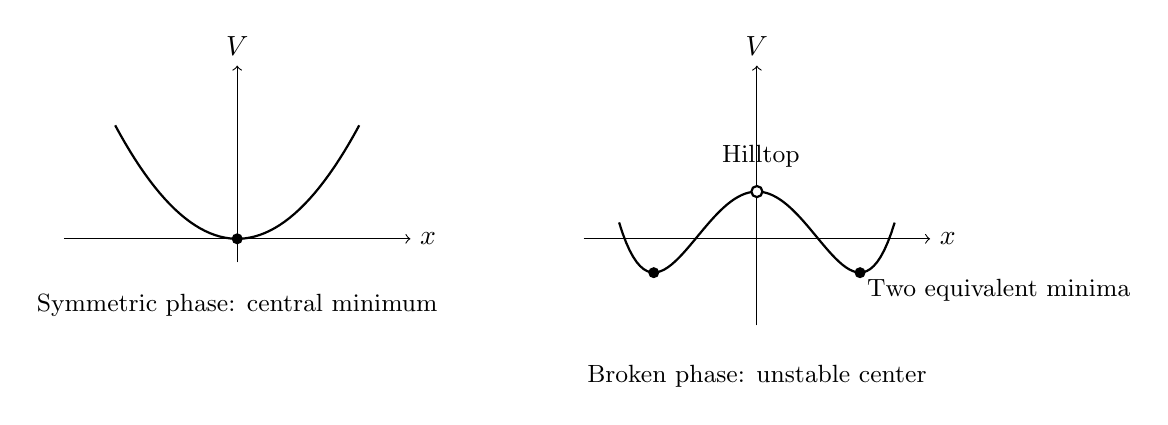
\begin{tikzpicture}[scale=1.0]
  % Left: single well, symmetric phase
  \draw[->] (-2.2,0) -- (2.2,0) node[right] {\(x\)};
  \draw[->] (0,-0.3) -- (0,2.2) node[above] {\(V\)};
  \draw[thick,domain=-1.55:1.55,samples=50] plot (\x,{0.6*\x*\x});
  \fill (0,0) circle (2pt);
  \node at (0,-0.85) {\small Symmetric phase: central minimum};
  % Right: double well, broken phase
  \begin{scope}[xshift=6.6cm]
  \draw[->] (-2.2,0) -- (2.2,0) node[right] {\(x\)};
  \draw[->] (0,-1.1) -- (0,2.2) node[above] {\(V\)};
  \draw[thick,domain=-1.75:1.75,samples=80] plot (\x,{-1.2*\x*\x+0.35*\x*\x*\x*\x+0.6});
  \fill (-1.31,-0.43) circle (2pt);
  \fill (1.31,-0.43) circle (2pt) node[below right=-1pt] {\small Two equivalent minima};
  \draw[fill=white,thick] (0,0.6) circle (2pt);
  \node at (0.05,1.05) {\small Hilltop};
  \node at (0,-1.75) {\small Broken phase: unstable center};
  \end{scope}
\end{tikzpicture}
\end{center}

\begin{mainline}
\textbf{A numerical estimate: how soon does a pencil fall?} An upright pencil is an inverted pendulum. A small angular deviation grows exponentially with characteristic time \(\tau\approx\sqrt{l/g}\). Take length \(l\approx 18\ \mathrm{cm}\) and \(g\approx 9.8\ \mathrm{m/s^{2}}\), giving \(\tau\approx\sqrt{0.18/9.8}\approx 0.14\ \mathrm{s}\). If release leaves only \(1\ \mathrm{mm}\) tip displacement, reaching visibly obvious \(10\ \mathrm{cm}\) requires \(100\)-fold amplification. Amplifying \(100\)-fold takes roughly \(\ln 100\approx 4.6\) characteristic times, or \(0.6\ \mathrm{s}\). This matches the experiment: better centering means longer waiting, but visible displacement quickly becomes an uncatchable fall. Notice the structure: waiting grows only logarithmically with initial precision. However perfectly you balance, you buy only fractions of a second of life. Perfectionism offers poor returns here.
\end{mainline}

\begin{mathbridge}
Why minima at \(x=\pm\sqrt{-a/(2b)}\)? Differentiate \(V(x)=ax^{2}+bx^{4}\):
\[
\frac{dV}{dx}=2ax+4bx^{3}=2x\,(a+2bx^{2})=0,
\]
giving \(x=0\) or \(x^{2}=-a/(2b)\), the latter real only for \(a<0\). The second derivative tests stability: \(V''(0)=2a\), so \(a>0\) gives a central valley and \(a<0\) a hilltop. One derivative translates phase transition into a sign change of \(a\).

Replace \(x\) by planar vector \((x,y)\), with potential depending only on distance from center:
\[
V=a\,(x^{2}+y^{2})+b\,(x^{2}+y^{2})^{2}.
\]
For \(a<0\), minima form not two points but a circle of radius \(\sqrt{-a/(2b)}\). Continuous rotation symmetry gives a continuous ring of equivalent broken ground states. Its cross-section resembles a Mexican hat. Moving around the ring costs no energy; only radial climbing out of the valley costs energy. This leads to an intuitive Goldstone theorem: whenever a continuous symmetry breaks spontaneously, a gentle, almost energy-free fluctuation along the valley must exist. Spin waves in magnets and sound in solids are such modes.
\end{mathbridge}

\begin{center}
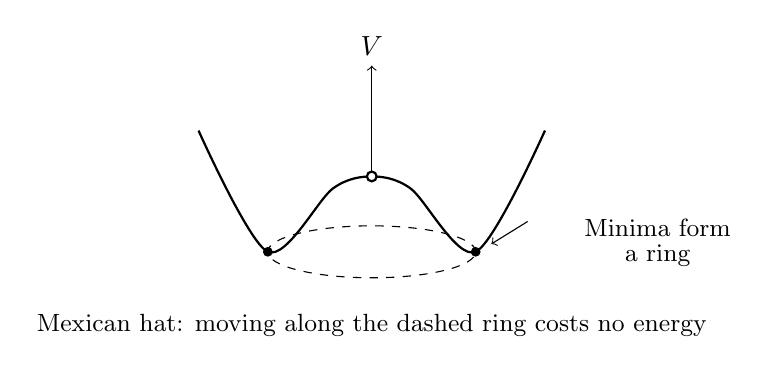
\begin{tikzpicture}[scale=1.1]
  % Mexican-hat section and top view of the valley ring
  \draw[thick] plot[smooth] coordinates {(-2,1.55) (-1.2,0.15) (-0.45,0.88) (0,1.02) (0.45,0.88) (1.2,0.15) (2,1.55)};
  \draw[dashed] (0,0.15) ellipse (1.2 and 0.3);
  \draw[->] (0,1.02) -- (0,2.3) node[above] {\(V\)};
  \fill (-1.2,0.15) circle (1.6pt);
  \fill (1.2,0.15) circle (1.6pt);
  \draw[fill=white,thick] (0,1.02) circle (1.6pt);
  \node at (3.3,0.25) {\small \shortstack{Minima form\\a ring}};
  \draw[->] (1.8,0.5) -- (1.38,0.24);
  \node at (0,-0.7) {\small Mexican hat: moving along the dashed ring costs no energy};
\end{tikzpicture}
\end{center}

\step{The Model's Limits}

\begin{mainline}
A good model states where it fails. Six boundaries follow: three establish validity and three warn against misleading explanations.

\textbf{First: states break symmetry, not laws.} Newton remains rotationally symmetric after a pencil falls; Maxwell still favors no direction after magnetization. No conservation law has been broken. Claiming symmetry is overthrown mistakes tearing a map for changing the territory.

\textbf{Second: a counterexample to perfect preparation preventing breaking.} Perhaps an ideal pencil, table, and vacuum would stand forever, making spontaneous breaking a cover-up for outside disturbance. Classically this is partly fair: an ideal inverted pendulum is an exact solution. Reality rejects it not through poor craftsmanship but quantum principles. A state cannot have both exact position, perfectly upright, and exact momentum, perfectly still. Uncertainty constrains states themselves, not crude instruments. Perfect undisturbed balance does not physically exist, so breaking needs no external excuse.

\textbf{Third: small systems restore symmetry.} A magnet of a few hundred atoms can choose a direction, yet thermal fluctuations or tunneling eventually reverse it back and forth; its average favors none. The strict mathematical fact is that a finite system's true ground state is often a symmetric superposition of all directions. Exact spontaneous breaking requires the infinite-size limit. Macroscopic magnets have roughly \(10^{23}\) atoms and reversal times far beyond the universe's age, justifying broken symmetry. Breaking concerns limits; everyday forever abbreviates longer than waiting for cosmic heat death.

\textbf{Fourth: do not oversell Higgs.} Chapter~59's gauge story continues here: modern theory has the space-filling Higgs field spontaneously fall from a symmetric state into a vacuum value, giving mass terms to \(W\), \(Z\), quarks, electrons, and other elementary particles while leaving photons massless. This explains elementary mass parameters' origins and why electromagnetic and weak interactions look different. It is not a universal weighing machine. Most body mass comes from protons and neutrons, whose mass is about ninety-nine percent quark--gluon interaction energy, largely unrelated to Higgs. Saying Higgs gives all matter its mass inflates a precise conceptual role into a beautiful misconception.

\textbf{Fifth: not every asymmetry is spontaneous breaking.} Hearts on the left, widespread right-handedness, or a river eroding one bank have particular causes, mostly historical accidents becoming established rather than symmetric-state instability. The concept has strict conditions: approximately symmetric laws, an unstable symmetric state, equivalent alternative states, and a sufficiently large system. Missing one should discourage automatic application. Beware the reverse misuse too: asymmetry does not prove biased laws, precisely the old view we dismantled.

\textbf{Sixth: names of directions are conventional; breaking's existence is not.} Naming magnetic poles or a battery's positive end is convention. A magnet selecting a direction is stability's physical requirement. Confusing these levels turns facts into cultural habits or habits into laws.
\end{mainline}

\begin{challenge}
\textbf{Finite-system symmetry restoration and Schr\"odinger's cat.} A quantum particle in a double well has a ground state not on one side but superposed across both. Tunneling connects the valleys and restores symmetry. Only infinitely many degrees of freedom suppress inter-state tunneling exponentially to zero, making superposition effectively equivalent to choosing one side. Macroscopic magnetic orientation is stable because astronomical numbers of microscopic degrees of freedom collectively take sides. This explains breaking's recurring association with macroscopic systems, condensation, and many degrees of freedom.

\textbf{Goldstone's theorem, stated.} Spontaneously break a continuous symmetry with short-range interactions and arbitrarily low-energy excitations, Goldstone modes, necessarily appear. Sound phonons and ferromagnetic spin waves are examples. Higgs is special: the broken symmetry is gauge symmetry, and the gauge field absorbs would-be Goldstone modes as massive gauge bosons' longitudinal components. This makes \(W\) and \(Z\) heavy. We state roles without deriving them.
\end{challenge}

\step{Explaining the Opening Phenomena}

\begin{mainline}
Return to the opening's three mysteries using the new model.

\textbf{The pencil.} Equivalent tabletop directions mean symmetric laws. Uprightness solves the equations but is an unstable hilltop. After release, unavoidable tiny displacement amplifies exponentially, settling into a directional valley within fractions of a second. One fall is unpredictable because pre-amplification displacements decide it; repeated directions are uniform because those displacements favor none. Angular momentum does not appear from nowhere: the pencil's directional, random momentum averages to zero, while pencil plus Earth conserves the total. Noether has defended itself beautifully: rotationally symmetric laws cannot prescribe a falling direction. Fluctuations choose; laws amplify them into a settled outcome.

\textbf{The magnet.} At high temperature, thermal motion randomizes needles, leaving zero order parameter and a symmetric phase. Cooling through the Curie temperature, about \(770\ ^{\circ}\mathrm{C}\) for iron and reachable with a candle flame, destabilizes symmetry. Alignment tendencies amplify and magnetization grows spontaneously, its direction chosen by fluctuations or residual fields during cooling. Reheating restores symmetry, explaining why red-heated and cooled magnets often acquire different pole directions.

% BEGIN TRANSLATOR SAFETY NOTE
\textbf{Translator safety note:} Do not use a candle or other flame to heat a magnet. The quoted iron temperature does not make this safe for refrigerator or neodymium magnets, coatings, or binders. Use a professionally prepared demonstration; see \href{https://www.kjmagnetics.com/faq.asp}{K\&J Magnetics' heating warnings}.
% END TRANSLATOR SAFETY NOTE

\textbf{Freezing and snowflakes.} Liquid water treats every direction equally: rotating the basin by any angle leaves it indistinguishable. Freezing forms a lattice with selected crystal axes, reducing continuous rotation symmetry to discrete sixfold symmetry. This downgrades rather than erases symmetry: ice retains integer multiples of sixty degrees. Snowflake branches are its traces, microscopic sixfold axes magnified by growth into visible patterns. No two flakes in one snowfall match because slightly different temperature and humidity histories amplify fine details into different branches. They share the same sixfold framework because laws allow it. One flake joins symmetry, breaking, and amplification.

\textbf{World structure.} We can answer the large opening question: uniformity and symmetry belong to laws and high temperature; structure and preference to solutions and low temperature. Galaxies, snowflakes, magnets, and elementary mass spectra are structures grown as laws cool into various broken phases. Symmetry is not richness's enemy: equivalent solution families give the world an opportunity to choose. Symmetry determines what may happen; breaking determines what does.

This prepares Chapter~61's two explanatory directions, fundamental and emergent. Broken-phase rules, such as sound speed or domain boundaries, need not be read word for word from microscopic equations; they arise from collective choices of many degrees of freedom. Microscopic symmetry nevertheless determines permitted choices. The two directions meet here.
\end{mainline}

\step{Thought Experiments and Challenges}

\begin{thought}[The Universe as a Cooling Pencil]
Today's particle-physics picture begins with an extremely hot early universe where electromagnetic and weak interactions belonged to one family under unified symmetry. Expansion and cooling let the space-filling Higgs field fall into a vacuum value, like a pencil falling or a magnet cooling. Unified symmetry breaks spontaneously: \(W\) and \(Z\) become heavy, photons remain massless, and electromagnetic and weak behavior diverge.

If the universe extends far beyond what we observe, might regions fall in different directions? Theory says possibly. Like magnetic domains or misoriented ice crystals, early cosmic breaking could choose inconsistently across space, leaving boundary defects called domain walls or cosmic strings. Searching for these ancient scars is a window into modern cosmology.

A deeper lesson follows: breaking erases part of its history. An inhabitant within a magnetic domain cannot infer locally what an unbroken world would have been, just as today's magnet cannot reveal its former directionless state. Cosmological observations are precious because Big Bang afterglow may preserve information from the instant of breaking, fingerprints of the world's choice.

\textbf{What it resembles:} cooling, instability, random choice, and domain boundaries are structurally like a cooling magnet. \textbf{What it does not:} the universe has no table or hand; its field fills all space without an external reference, and its direction is internal field orientation, not a spatial compass bearing. Do not literally imagine a cosmic pencil on a table.
\end{thought}

\begin{mainline}
These four questions emphasize reasoning, not calculation. Each has a hint, but think first. They follow four steps: discrete versus continuous, quantitative instability, breaking and structure, and experimental order-parameter criteria.

\begin{puzzles}
  \item Release an upright coin and it falls; release an upright pencil and it falls too. How do these symmetry breakings fundamentally differ? Hint: count equivalent outcomes and recall continuous breaking's almost energy-free slow fluctuations. Does the coin have one?
  \item Someone says a perfect pencil on a perfect table with no disturbance never falls, making spontaneous breaking unnecessary. Give two independent objections. Hint: one concerns stability and waiting time's dependence on initial displacement; the other concerns quantum limits on states. Does exactly upright and exactly still exist?
  \item Liquid water favors no direction, while ice chooses axes and has less symmetry. Why can less symmetric ice produce such regular, rich snowflake patterns? Hint: how many choices does the symmetric phase offer, and how many the broken phase? What does structure require?
  \item Heat an iron nail red-hot and quickly bring it near a compass, assuming no contact or heat damage. Does the compass noticeably deflect? Try again after cooling. Hint: consider the order parameter above and below Curie temperature. No macroscopic magnetism is not the same as no response to a magnetic field; paramagnetic response persists but is weak.

% BEGIN TRANSLATOR SAFETY NOTE
\textbf{Translator safety note:} Do not heat a nail in a household flame or carry red-hot metal toward a compass. Treat this as a thought experiment or view an instructor's recorded demonstration. Hot metal and open flames require controlled laboratory procedures; see \href{https://institute.acs.org/acs-center/lab-safety/education-training/safer-experiments/flame-test.html}{American Chemical Society flame-demonstration safety guidance}.
% END TRANSLATOR SAFETY NOTE
\end{puzzles}
\end{mainline}
